\begin{frame}{Concrete Example: Fairness in hiring decisions \cite{barocas-hardt-narayanan}}
\begin{columns}
\begin{column}{0.5\textwidth}
   \begin{itemize}
       \item In reality: non-linear model
       \item Two demographic groups: \textbf{triangles} and \textbf{squares}
       \item No consideration about group assignment
       \item Still: Triangles are higher performing and are more positively classified
   \end{itemize}
\end{column}
\begin{column}{0.5\textwidth}  %%<--- here
    \begin{figure}
        \centering
        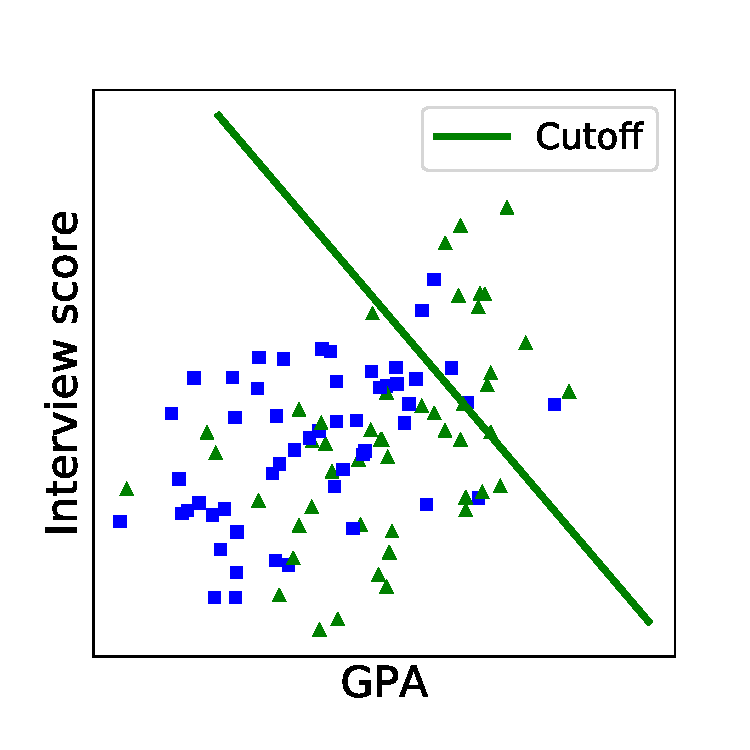
\includegraphics[width=.70\textwidth]{presentation/assets/toy_example.pdf}
        \caption{Hiring classifier that predicts job performance (not shown) based on GPA and interview score with a cutoff \cite{barocas-hardt-narayanan}}
        \label{fig:example1}
    \end{figure}
\end{column}
\end{columns}
\end{frame}

\begin{frame}{Concrete Example: Fairness in hiring decisions \cite{barocas-hardt-narayanan}}
    \begin{columns}
\begin{column}{0.5\textwidth}
\underline{\textbf{Reasons for Disparities:}}\newline 

   \begin{itemize}
       \item Managers who score performance might have bias against one group
       \item Workplace biased, preventing group from reaching their full potential
       \item Disparities in educational institutions attended
   \end{itemize}
\end{column}
\begin{column}{0.5\textwidth}  %%<--- here
    \begin{figure}
        \centering
        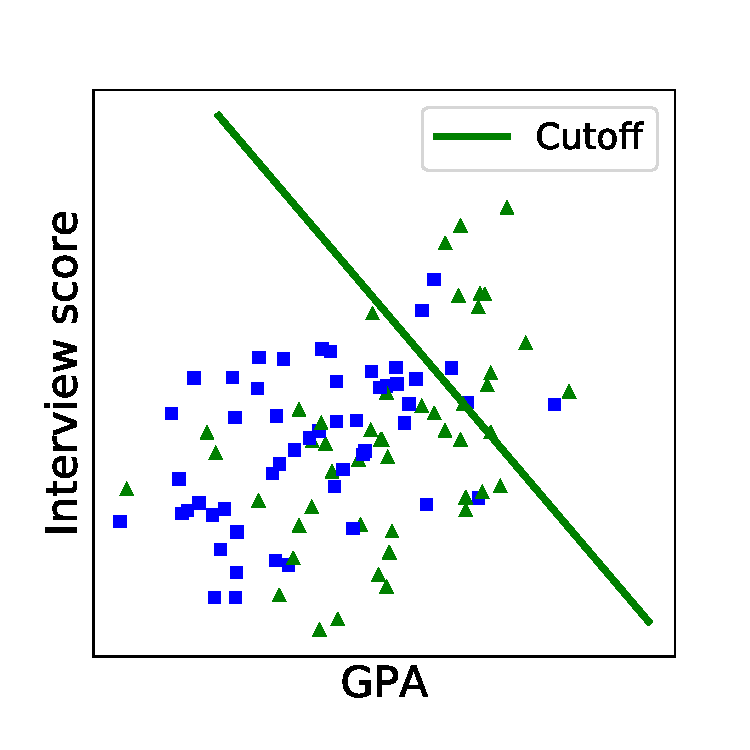
\includegraphics[width=.70\textwidth]{presentation/assets/toy_example.pdf}
        \caption{Hiring classifier that predicts job performance (not shown) based on GPA and interview score with a cutoff \cite{barocas-hardt-narayanan}}
        \label{fig:example2}
    \end{figure}
\end{column}
\end{columns}
\end{frame}

\begin{frame}{Concrete Example: Fairness in hiring decisions \cite{barocas-hardt-narayanan}}
    \begin{columns}
\begin{column}{0.5\textwidth}
\underline{\textbf{Solving unjustified Disparities:}}\newline 

   \begin{itemize}
       \item GPA proxy for demographic group (dropping it would result in a loss of accuracy)
       \item Using different cutoffs for hiring so both groups have same probability of being hired (which cutoffs?)
       \item \underline{Generally:} Many algorithmic possibilities especially \textbf{similarity function between pairs of individuals}
   \end{itemize}
\end{column}
\begin{column}{0.5\textwidth}  %%<--- here
    \begin{figure}
        \centering
        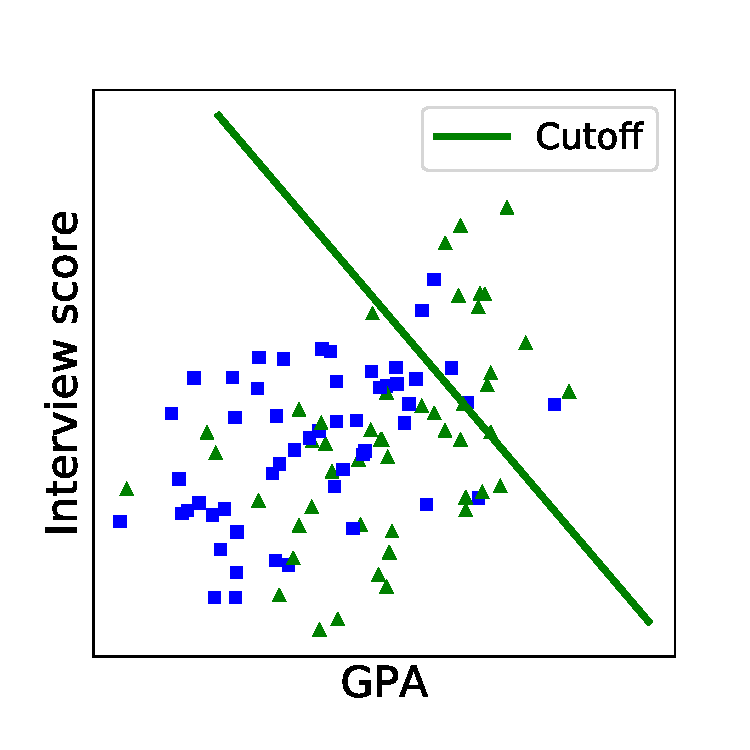
\includegraphics[width=.70\textwidth]{presentation/assets/toy_example.pdf}
        \caption{Hiring classifier that predicts job performance (not shown) based on GPA and interview score with a cutoff \cite{barocas-hardt-narayanan}}
        \label{fig:example3}
    \end{figure}
\end{column}
\end{columns}
\end{frame}